\section{Kubernetes security automation}
\label{sec:kubernetes-security-automation}

This section introduces the reader to the topic of the security automation inside the Kubernetes cluster. We discuss different security tools, their place in the cloud Infrastructure and examine their usage patterns. Additionally, we explain why were the specific tools chosen for our research.

\subsection{Overview}

Kubernetes security scanners and operators provide an array of defensive capabilties. Most of them act in the form of informator. That is, they do not perform any remediatory actions, but only provide user with information about the cluster security status. Nevertheless, there are some solutions on the market that are capable of resolving some of the security issues automatically. This, on the other hand, introduces another layer of concern: can we really trust a third-party system to introduce modifications to our infrastructure? That the former type is the most abundant and is the focus of this paper. Automatic remediation can be then implemented as a part of CI/CD pipeline based on the scan results. This ensures that it is compliant with the company's policies and is tailored to the company's needs.

One of the ways to classify Kubernetes security scanners is by the scan target. Here we can roughly divide them into three groups: configuration file scanners, cluster scanners and container image scanners. Most of the tools, however, can be put into multiple different groups. Cluster scanners usually are able to perform container image scanning as well and it is a part of the full cluster scan. Cluster scanners detect misconfigurations in the cluster infrastructure and its essential components. They look for, among other things, containers running with extensive privilages, exposed sensitive workloads and plaintext secrets. Container image scanners look for known vulnerabilities inside the images. Configuration file scanners perform a scan of the cluster configuration files. For large infrastructure with a number of applications deployed there might be over several tens of thousands lines of configuration and such scanners aim to detect any known misconfigurations by going through theese lines.

Cluster security scanners can be further classified by the execution point. Again, there is usually more than one way to run a scan, but here are a few options: run a scanner tool as a container, run it from a remote machine connected to the cluster, run it is an operator, which can perform scan automatically on a regular basis. To always keep cluster up-to-date with the most recent security patches the best solution would be to either install an operator or integrate a security scanner tool into your CI/CD pipeline.

\subsection{Selection Criteria}

To perform our assessment we have chosen from a variety of Kubernetes security scanners. Though the area is still relatively new, there is a variety of tools with different purposes available on the market. We made our choice based on the following criteria:
\begin{itemize}
\item \textbf{free-to-use} \\
We do include some proprietary tool testing further in our research as an additional comparison, however, for the main part we only use free tools. Kubernetes itself is distributed under Apache License 2.0, which means it is inherently free to use. The ability to adopt these tools without financial constraints enables wider adoption, thus, contributing to the community-driven innovations. Finally, this research not being funded, we could only afford to work with openly distributed software.
\item \textbf{open-source} \\
Again, we are sticking to the open-source nature of the Kubernetes. By selecting open-source tools, this research ensures that each tool's codebase is transparent and can be reviewed by security experts. This transparency increases trust in the tools' effectiveness, as the community can spot, disclose, and even patch any vulnerabilities in the software. Another advantage is the customization of the open-source software as the companies can adapt the tools to their specific Kubernetes security needs.
\item \textbf{designed with cloud in mind} \\
Designed to be used in the Kubernetes environment specifically, these tools should offer features like scanning container images for vulnerabilities, but also monitoring network policies, securing Kubernetes configuration files, or identifying misconfigurations within clusters. Tools built specifically for Kubernetes are more efficient, as they are optimized to address the distinct aspects of the platform, making security management more effective.
\item \textbf{has an active community support} \\
Tools with active communities tend to have more frequent updates, faster response times for bug fixes, and a wide range of contributors who bring diverse insights to improve functionality and security. The world of the software security is changing rapidly and an active community means that the tool is up-to-date with the most recent events. A thriving community also means that users can easily access support on the community forums.
\end{itemize}

Based on the aforementioned criteria we ended up choosing and testing the following tools:
\begin{itemize}[noitemsep]
\item Trivy
\item Kube-bench
\item Prowler
\item Kubescape
\end{itemize}

In the next chapters we closely examine each selected tool and explain how it is matches our selection criteria. Additionally, we compare them to each other and highlight their strong and weak sides.

\subsection{Trivy}
Trivy is an Aqua Security open source project with a vast array of use cases. It supports multiple scan targets and includes multiple scanners. Among the supported targets are:
\begin{itemize}[noitemsep]
    \item Container Image
    \item Filesystem
    \item Git Repository 
    \item Virtual Machine Image
    \item Kubernetes
\end{itemize}
Trivy includes scanners for:
\begin{itemize}[noitemsep]
    \item OS packages and software dependencies in use (SBOM)
    \item Known vulnerabilities (CVEs)
    \item IaC issues and misconfigurations
    \item Sensitive information and secrets
    \item Software licenses
\end{itemize}

According to the Trivy official Gihub page \cite{trivy-github}, it can be installed on the local machine using any of the popular package mangager or by downloading a binary from the Github Releases. It can also be ran as a Docker container or Kubernetes Operator. Furthermore, Trivy can be integrated into GitHub Actions or installed as a Visual Studio Code plugin. Aqua Security uploads each new release as a Docker image into the Dockerhub repository. There is a variety of supported configuration parameters for Trivy Kubernetes scanning feature. Users can specify which scanners to include, which namespaces to skip, which nodes to scan and the format of the output. An example of a Trivy misconfiguration scan command executed against the default Kubernetes context, which would output a short summary of findings and skip \textbf{dev-system} namespace, is included below (see Listing~\ref{lst:trivy-k8s}).

\begin{center}
    \begin{lstlisting}[language=bash, caption={[An example of a Trivy Kubernetes scan command] An example of a Trivy Kubernetes scan command.}, label={lst:trivy-k8s}]
    $ trivy k8s \
        --scanners=misconfig \
        --report=summary \
        --exclude-namespace=dev-system
    \end{lstlisting}
\end{center}

Since Kubernetes is listed as a natively supported target and Trivy can scan for both vulnerabilities and misconfigurations, Trivy is well-suited for our research. It is also open source and available for free. Presently, Trivy's Github repository has over 2800 issues, with a little over than 150 of them being open, repository's commit history shows active development with a bi-monthly minor release cycle and yearly major release cycle. Thus, we can assume an active community and developer support.

\subsection{Kube-bench}
Kube-bench is another open source tool developed by Aqua Security. Their Github page \cite{kube-bench-github} states that it checks whether Kubernetes is deployed securely by running the checks against the CIS Kubernetes Benchmark (see \ref{sss:cis-kubernetes-benchmark}). Kube-bench is designed specifically for Kubernetes. Users can run the it inside a Docker container or deploy it as a Kubernetes job, however, there is still an option to download the binary on the local machine and run it against the desired Kubernetes cluster.

Since kube-bench has a much narrower feature set than Trivy, it is much more simple in usage, but still highly configurable. Configuration can be supplied via a config file or we can pass the configuration parameters directly using one of the 24 flags. An example of a simple scan command targeting \textbf{master}, \textbf{node}, \textbf{etcd}, \textbf{policies} CIS Benchmark categories is provided in Listing~\ref{lst:kube-bench-scan}.

\begin{center}
    \begin{lstlisting}[language=bash, caption={[An example of a Kube-bench scan command] An example of a Kube-bench scan command.}, label={lst:kube-bench-scan}]
    $ kube-bench run \
        --targets master,node,etcd,policies
    \end{lstlisting}
\end{center}

Kube-bench is actively supported by the developers and the community. At the present moment, Kube-bench Github repository has about 500 issues, 10\% of which are currently open. Repository receives updates on a weekly basis and the new version is released monthly.

\subsection{Prowler}

Prowler, as described on the Github page \cite{prowler-github}, is an open source security tool designed to perform Kubernetes security best practices assessments, audits, incident response, continuous monitoring, hardening and forensics readiness, and remediation. It is shipped with a built-in dashboard, which displays scan results in graphical format (see Fig~\ref{img:prowler-dashboard}). However, the dashboard can only read the scan results from the folder on the host machine and the user cannot trigger a new scan directly from the dashboard. Users have to install a separate Prowler App inside the clusters to trigger the scan. According to the documentation \cite{prowler-app-page}, ``it provides a user-friendly interface to configure and run scans, view results, and manage your security findings.''

\begin{figure}[!hbt]
	\begin{center}
		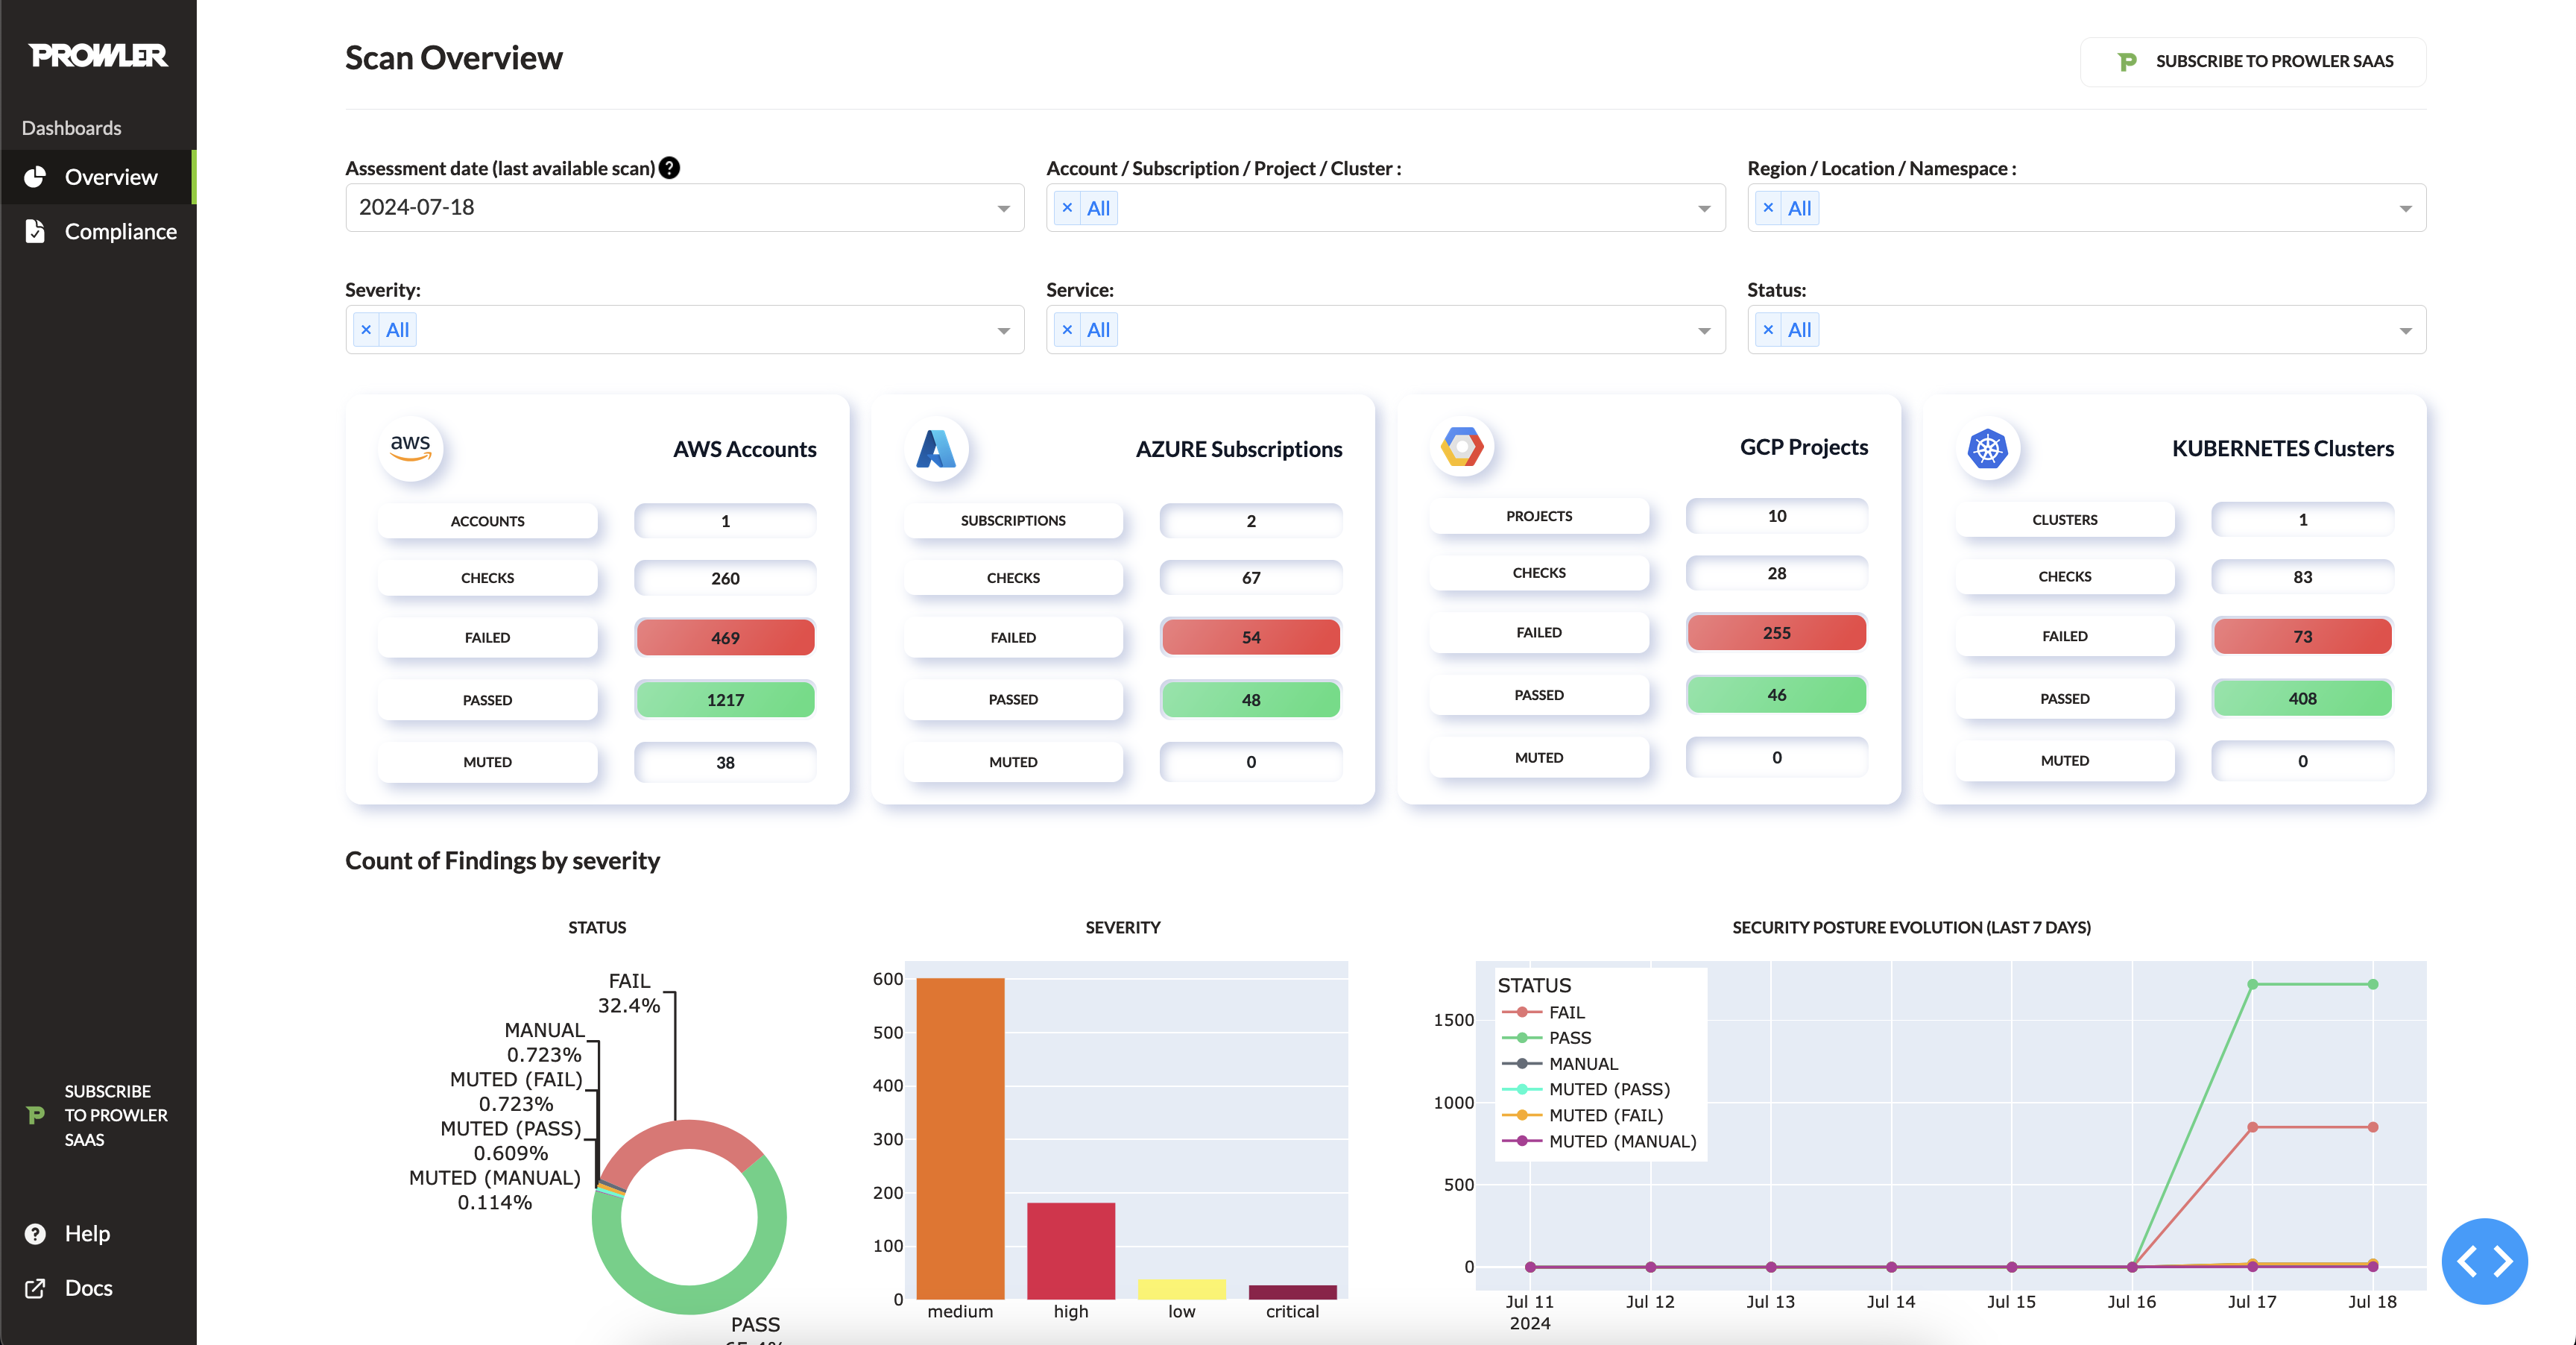
\includegraphics[width=0.85\textwidth]{images/prowler-dashboard.png}
        \caption{Prowler dashboard interface.}
		\label{img:prowler-dashboard}
	\end{center}
\end{figure}

Prowler CLI supports Azure, Google Cloud, AWS and generic Kubernetes providers. It performs a scan against multiple Kubernetes security frameworks to ensure the best coverage. Prowler supports output in CSV or JSON-OCSF format, the latter being an independent open source developed JSON schema by Open Cybersecurity Schema Framework project, which has recently joined the Linux Foundation organization. Again, we configure the Prowler job either via a configuration file or by passing the flags directly in the execution command. Listing~\ref{lst:prowler-command} provides an example on how can a Prowler scan be triggered. This particular execution would output the results in \textbf{json-ocsf} format, including only failed and manual checks.

\begin{center}
    \begin{lstlisting}[language=bash, caption={[An example of a Prowler scan command] An example of a Prowler scan command.}, label={lst:prowler-command}]
    $ prowler kubernetes \ 
        --status FAIL,MANUAL \
        --output-formats json-ocsf
    \end{lstlisting}
\end{center}

There are over a thousand issues in official Prowler Github repository. The development is still in progress and the tool receives regular updates. The project has an active community with operational development support.

\subsection{Kubescape}
Kubescape is an open-source security platform designed to harden the security of a Kubernetes cluster. Kubescape CLI allows users to scan the cluster from the local machine. Kubescape Operator enables image vulnerability scanning as well as continuous and scheduled scanning. Kubescape also offers Github Actions integration for CI/CD pipelines according to the official Github page \cite{kubescape-github}.

Kubernetes cluster is verified against a posture library (available at Github \cite{regolibrary-github}), which is a collection of frameworks each containing a set of controls. By default, the library is comprised of NSA Framework controls, MITRE ATT\&CK Framework controls and CIS Benchmark controls.

Scan configuration is again passed with multiple flags. There are flags allowing to select the namespaces to include into scan, namespaces to exclude from the scan, output format and location. Scanning can be then performed using the command displayed in Listing~\ref{lst:kubescape-command}.

\begin{lstlisting}[language=bash, caption={[An example of a Kube-bench scan command] An example of a Kube-bench scan command.}, label={lst:kubescape-command}]
    $ kubescape scan \
        --format json \
        --output kubescape-scan.json
\end{lstlisting}

Kubescape's repository shows ongoing development with regular update releases.

\subsection{Preliminary Comparison}

This section compares the selected tools based on their declared feature set, ease of installation and execution, scan targets, supported cloud providers and security frameworks. This comparison does not include the analysis of the scan results, performance or any other aspects of execution. A detailed analysis of the generated reports can be found in Chapter~\ref{chap:results}.

We start by comparing the scanners by their feature set. Trivy has the most broad feature set as it is able to scan for vulnerabilities inside the images, perform IaC scan (supporting Terraform, Helm, plain Kubernetes YAML), scan for misconfigurations in Kubernetes resources and generate SBOM. Kube-bench is designed to perform only two tasks: CIS Kubernetes Benchmark checks and Node-level audit, making it very specialized tool. Prowler is able to detect misconfigurations and security threats, perform CIS Benchmark checks and cloud security audit. Kubescape's features include misconfiguration and container vulnerability scanning, RBAC risk analysis and SBOM generation. While all of the scanners can detect Kubernetes misconfigurations, only Trivy and Kubescape have the ability to scan for the vulnerabilities in containers. SBOM generation is a requirement for enterprise-level scanners nowadays, which makes Kubescape and Trivy stand out once again.

When we compare the tools by the supported cloud providers, simplicity of Kube-bench makes it the leader in this category. Since Kube-bench only performs static analysis, this makes it cloud agnostic, meaning that it can be used with any cloud provider as long as the provider offers Kubernetes services. Trivy, Kubescape and Prowler all support the same cloud providers. Kubescape and Trivy both natively support AWS, Azure and GCP. Prowler's focus is AWS, but it also supports Azure and Google Cloud Platform.

All of the presented tools declare full CIS Benchmark coverage, which is the only supported framework for Kube-bench. Trivy additionally declares NSA and MITRE ATT\&CK coverage. Kubescape further extends the set with NIST 800-53 and SOC 2 frameworks, which are more specialized frameworks, the former developed by the U.S. government and focuses on technical and administrative controls, while the latter focuses on the customer data security and compliance. Prowler mixes the CIS Benchmark checks with the four major security and privacy frameworks or regulations relevant to organizations handling sensitive data (PCI-DSS, GDPR, HIPAA, ISO27001).

From the user perspective we can compare the scanners by the ease of installation and execution. Trivy's binary is available for download using most of the popular package managers (like Brew for MacOS and apt-get, yum, pacman and others for various Linux distros). Less secure but more convenient way of installation is by using a script. Additionally, Trivy has a Docker image available in Docker Hub, GitHub Container Registry and AWS Elastic Container Registry. Trivy can be executed against an active Kubernetes context using the binary or installed as an operator inside the cluster for automatic scanning every six hours. Kube-bench is similar in installation process to the Trivy. However, Kube-bench Docker image is compiled for linux-x86-64 only. Kube-bench also provides a \textbf{job.yaml} file, which can be used to run it inside the cluster as a Kubernetes Job. Kube-bench runs checks specified in controls files that are a YAML representation of the CIS Kubernetes Benchmark checks. Kubescape supports the usual installation channels. Additionally, users are able to download scan artifacts (frameworks) separately. Kubescape Operator can be installed inside the using a Helm chart. Unfortunately, Kubescape Operator must be installed in the cluster for the Kubescape CLI to be able to scan for vulnerabilities. Prowler CLI can be installed only as a Python module, but there are also Docker images available to download from the Docker Hub and AWS Public ECR. Prowler also provides an applciation, which displays scan results in a graphical format. Table~\ref{tab:preliminary-scanner-comparison} summarizes our preliminary comparison findings.

\begin{table}[H]
    \begin{center}
        \begin{tabular}{
            | >{\raggedright\arraybackslash}p{.15\textwidth} 
            | >{\raggedright\arraybackslash}p{.22\textwidth} 
            | >{\raggedright\arraybackslash}p{.15\textwidth} 
            | >{\raggedright\arraybackslash}p{.20\textwidth} 
            | >{\raggedright\arraybackslash}p{.15\textwidth} | }
        \hline
        \textbf{Tool} & \textbf{Features} & \textbf{Cloud support} & \textbf{Frameworks} & \textbf{User experience} \\
        \hline\hline
        Trivy & Vulnerability scan, Misconfiguration scan, IaC scan, SBOM generation, Operator & AWS, Azure, GCP & CIS, NSA, MITRE ATT\&CK & CLI tool \\
        \hline
        Kube-bench & CIS Benchmark audit & cloud agnostic & CIS & CLI tool \\
        \hline
        Prowler & Cloud audit, misconfiguration scan, compliance scan, Operator & AWS, Azure, GCP & CIS, PCI-DSS, GDPR, HIPAA & CLI tool, UI app \\
        \hline
        Kubescape & Operator, misconfiguration scan, vulnerability scan, SBOM generation, RBAC analysis & AWS, Azure, GCP & CIS, NSA, MITRE ATT\&CK, NIST 800-53, SOC 2 & CLI tool \\
        \hline
        \end{tabular}
    \end{center}
    \caption{Kubernetes security scanners preliminary comparison.}
    \label{tab:preliminary-scanner-comparison}
\end{table}